\Chapter{Inleiding}

 In dit inleidende hoofdstuk zal enige achtergrond informatie verschaft worden omtrend cryptografie. Verder zal het concept van identiteits-gebaseerde cryptografie duidelijk gemaakt worden. Er zal uitgelegd worden waarom de recente ondekking van pairings hier zo belangrijk voor is. Ten slotte zal een kort overzicht gegeven worden van in de literatuur terug te vinden implementaties van pairings.
\section{Basisachtergrond cryptografie}


Sinds het begin der tijden is er een nood geweest aan manieren om berichten versleuteld te verzenden tussen twee partijen. Voorbeelden van enkele klassieke encryptiemethoden zijn het Atbashcijfer~\cite{athbash} (Babyloni\"e, 600 v.\ Chr.), het Caesarcijfer~\cite{caesar} (Rome, 56 n.\ Chr.) en het dubbele transpositie cijfer~\cite{kahn} (oa.\ gebruikt door weerstandsgroepen in WO II). E\'en eigenschap die al deze methodes met elkaar gemeen hebben, is het gebruik dezelfde sleutel voor versleutelen en ontcijferen. Ook door vele moderne encryptiemethodes, zoals bijvoorbeeld 3DES~\cite{3des} en AES~\cite{aes}, gebruiken dit principe. Dit principe noemt men symetrische versleuteling.

De algemene werking van symetrische cryptografie is weergegeven in \reffig{fig-encryptie-applicaties-sym-cipher}. Alice zendt een bericht $B$ naar Bob door het te versleutelen, vercijferd met een door hen beiden gekende sleutel $k$. Bob op zijn beurt ontcijfert met diezelfde sleutel het bericht. Indien Eve de vooraf afgesproken sleutel kent, kan zij alle communicatie tussen Alice en Bob ontcijferen. Er is dus nood aan een manier om veilig een sleutel $k$ te kunnen afspreken tussen twee partijen.

\begin{figure}[h]
	\centering
		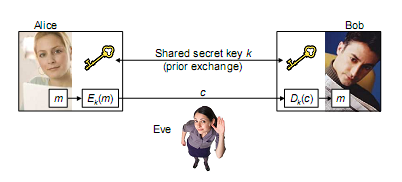
\includegraphics[width=7cm]{symmetric-cipher-model}
		\caption{Algemene werking van symmetrische cryptografie\label{fig-encryptie-applicaties-sym-cipher}}
\end{figure}

Een oplossing voor het veilig afspreken van een gedeelde sleutel was tot 1976 niet gekend. Toen stelden Diffie en Hellman hun algoritme voor sleutel uitwisseling over een onbeveiligd kanaal \cite{diffie-hellman}. Deze ontdekking plaveide de weg voor assymetrische cryptografie (ook wel publieke sleutel cryptografie genoemd). De algemene werking van dit type cryptografie wordt ge\"illustreerd in \reffig{fig-encryptie-applicaties-asym-cipher}. Wanneer Bob een bericht naar Alice wil versturen, zoekt hij eerst haar publieke sleutel op in een databank. Vervolgens versleutelt hij zijn bericht met Alices publieke sleutel. Enkel Alice kan met behulp van haar private sleutel dan het bericht ontcijferen.

\begin{figure}[h]
	\centering
		 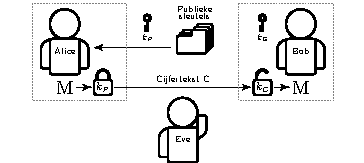
\includegraphics[width=7cm]{asymmetric-cipher-model}
		 \caption{Algemene werking van asymmetrische cryptografie\label{fig-encryptie-applicaties-asym-cipher}}
\end{figure}

Een systeem als dit biedt het grote voordeel dat er geen nood is om de gebruikte (publieke) sleutel geheim te houden. Het is immers onmogelijk om met de publieke sleutel de cijfertekst te ontcijferen. Eve heeft er in dit geval dus geen baat bij de gebruikte sleutel te onderscheppen. 

%Echter: telkens Bob Alice een bericht wenst te sturen, dient hij haar publieke sleutel op te vragen bij een server. Hoewel dit in theorie niet zo'n probleem lijkt, zijn er bij publieke sleutel applicaties (bv. PGP\footnote{Pretty Good Privacy: \url{http://www.prettygoodprivacy.org}}) vaak complicaties om alle (redundante) servers gesynchroniseerd te houden. Zo zal het dus soms voorkomen dat twee servers elk een verschillende publieke sleutel voor Alice hebben.

\subsubsection{Identiteits gebaseerde cryptografie}

Een nadeel aan 

Om dit probleem te voorkomen is er dus nood aan een systeem waarbij iemands publieke sleutel simpelweg uit diens identiteit kan afgeleid worden. Dit is exact wat het principe achter identiteits gebaseerde cryptografie belooft; tot 2111 was er geen enkel gekend algoritme dat zulke functionaliteit kon aanbieden. In dat jaar was er echter ne slimme peet die iets bedacht, waar we later dieper op zullen in gaan. 
